\section{Spatial Verification Methodology}

We examine the use of EMD for verifying spatial relationships.  We run our separate analyses on two separate
data sets.  The first is a data set at Todai and the other is a data set in Sutardja Dai Hall at UC Berkeley.
For the Todai data set, we use a simple methodology whereby we run a pairwise correlation analysis on the IMFs
for traces in that building.  We create clusters of traces that share a high correlation value and examine
the spatial characteristics of the clusters as we sweep through the acceptance threshold on the correlation
values.  

The second analysis is on a separate data set in Sutardja Dai Hall.  There, we expand the methodology from the Todai 
dataset and apply machine learning techniques to systematize the clustering processes.  We also examine
the effectiveness of our clustering algorithm as we sweep through a series of threshold values.
We present both methodologies and results in this section.

% \begin{figure}[tb]
% \hspace{-2cm}
% 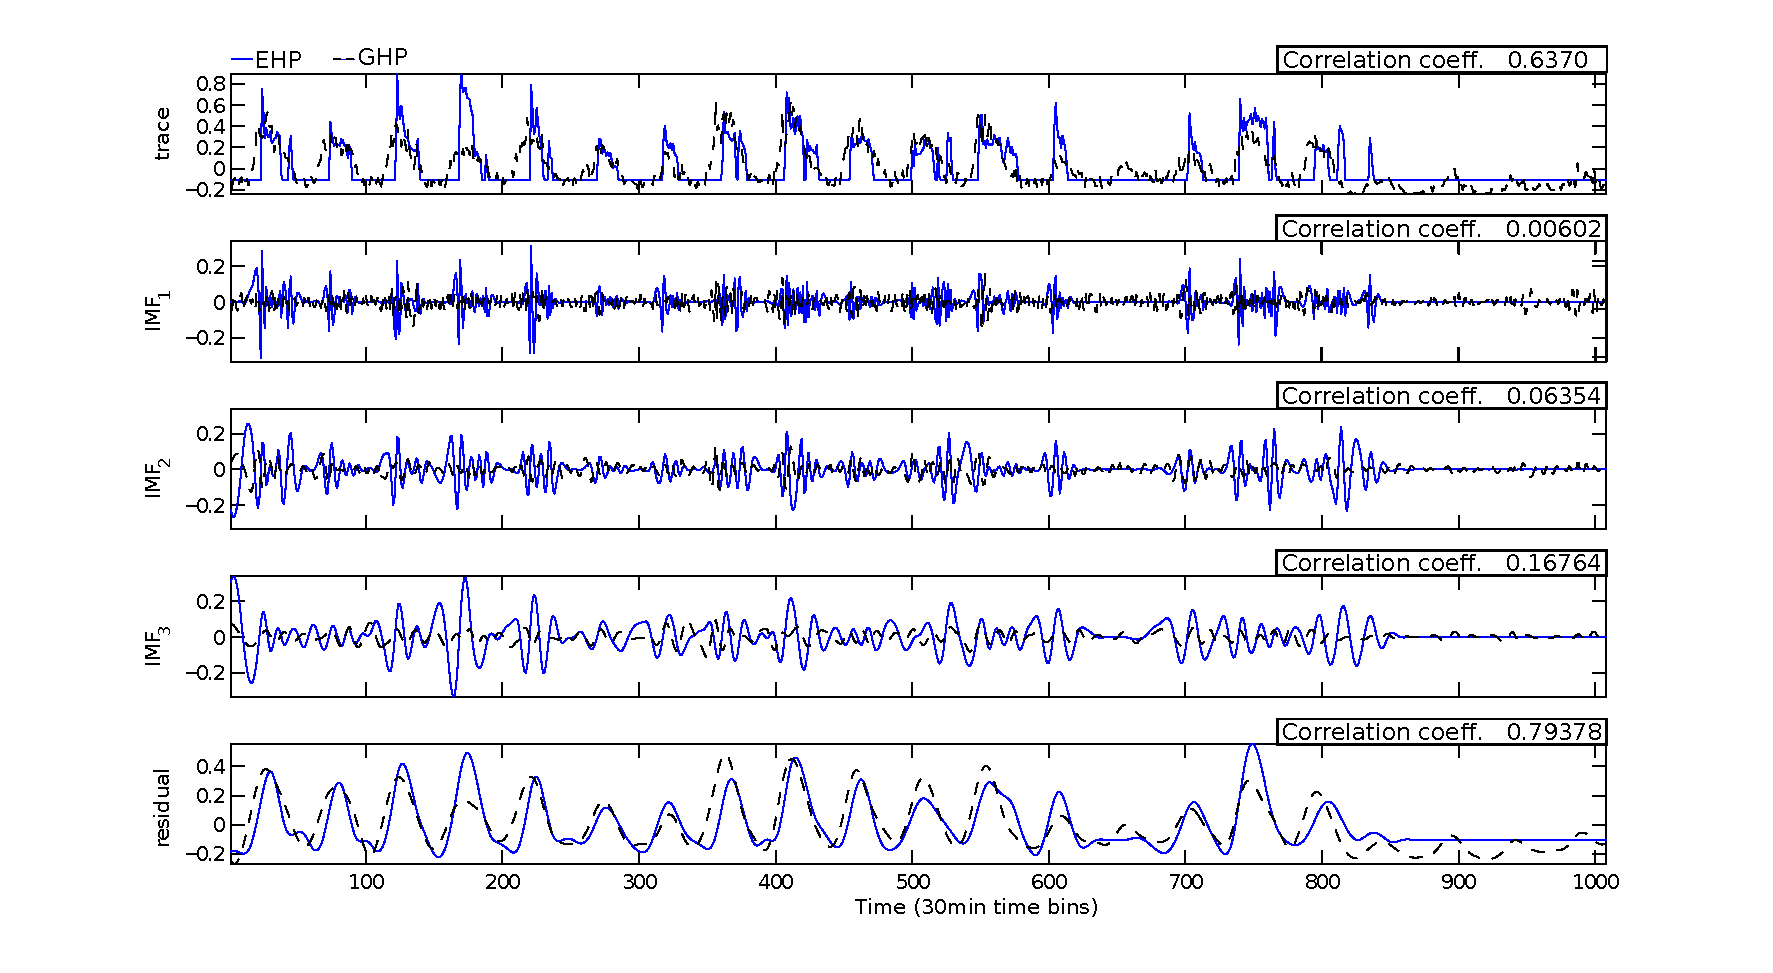
\includegraphics[width=1.2\textwidth]{figs/emd_25_41-eps-converted-to}
% \vspace{-1cm}
% \caption{Decomposition of the EHP and GHP trace using bivariate EMD. IMFs correlation coefficients highlight the intrinsic independence of the two traces.}
% \label{fig:emd2}
% \end{figure}


% \begin{figure}[ht!]
% \centering
% 	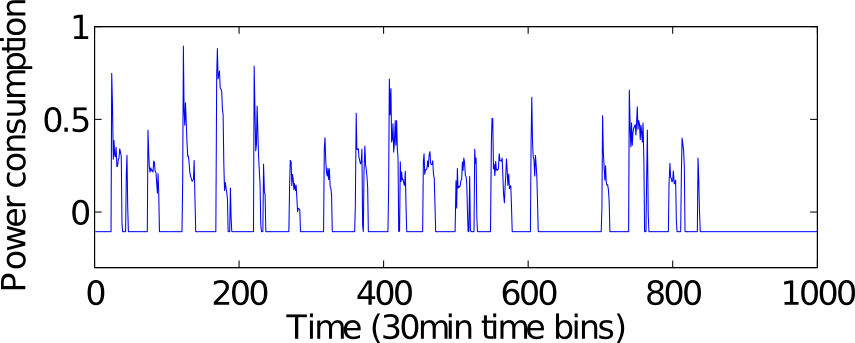
\includegraphics[width=.4\textwidth]{figs/25.png}
% \caption{Trace from an Electric Heat Pump (EHP) captured in 2011 from July 4th to July 24th. Data is 
% normalized and aggregated into 30 minutes time bins.}
% \label{fig:raw_ehp}
% \end{figure}

% \begin{figure}[ht!]
% \centering
% 	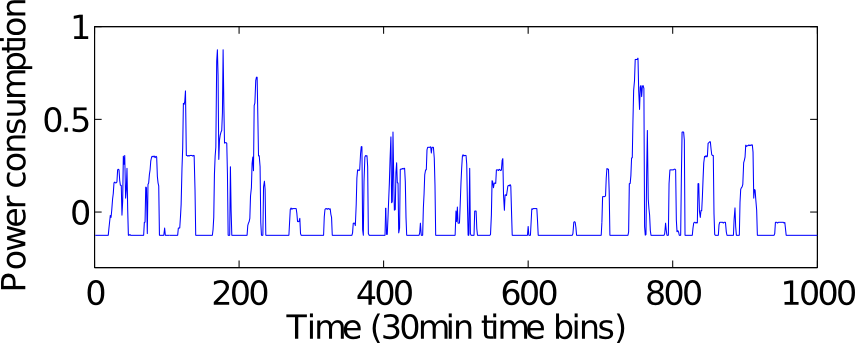
\includegraphics[width=.4\textwidth]{figs/26.png}
% \caption{Light traces from captured in 2011 from July 4th to July 24th. Data is 
% normalized and aggregated into 30 minutes time bins.}
% \label{fig:raw_light}
% \end{figure}

% \begin{figure}[ht!]
% \centering
% 	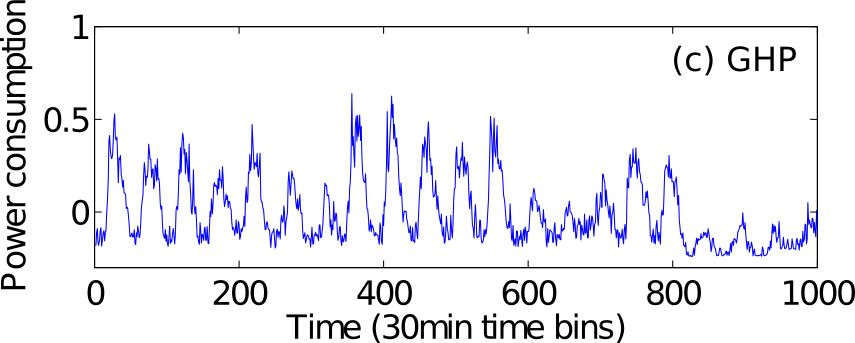
\includegraphics[width=.4\textwidth]{figs/41.png}
% \caption{Traces from a Gas Heat Pump (EHP) captured in 2011 from July 4th to July 24th. Data is 
% normalized and aggregated into 30 minutes time bins.}
% \label{fig:raw_ghp}
% \end{figure}

\subsection{Todai Data Set Analysis Methodology}
For the first investigation, we focus on a three-week span in the summer of 2011 (from July 4th to July 24th).
The dataset captures regular work days, weekends, and one holiday (July 18th).  This timeframe captures
the typical usage of the equipment, triggered by occupant activity.  For the initial
analysis, we focus on three sensors; two pumps -- eletric heat pump (EHP) and a gas heat pump (GHP) and a light feed,
that measure the light level is lumens.  
% The first pump is an 
% ``electric heat pump'' and is labled as EHP, the second  is a ``gas heat pump''
% and labeled as GHP.
The room lighting system serves the same room as the EHP.  The GHP
serves a different room on the same floor.  The expanded portion of this analysis pivots on the EHP
and does a pairwise comparison between it and all other sensors in the building.
% Computationally, this approach does not scale to a large number of sensors.  For future work, we will
% examine various heuristics to narrow the search space before running pairwise comparisons.
We use EMD to detrend each of the traces and pay particularly close attention to the high-frequency IMFs.  Our 
hypothesis is that correlating at the higher frequencies will yield more meaningful comparisons.
In buildings, metadata is poorly and unsystematically managed within a single system domain.  Moreover, 
with the ever growing number of additional sub-meters, it is important to quickly integrate
sensor data from multiple systems to understand the full state of the building.  It is also important to 
understand how sensors are used in concert.  Anomalies in usage may indicate underlying problems with 
the equipment or inefficient/incorrect usage.  


% \begin{figure}[t!]
% \centering
%  \subfigure[EHP trace]{\label{fig:raw_ehp}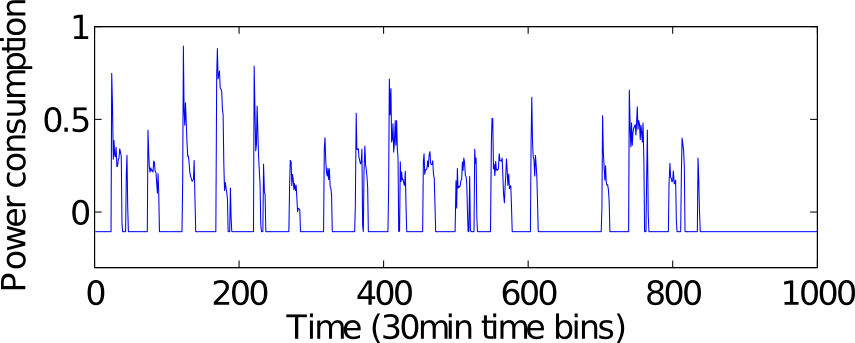
\includegraphics[width=.4\textwidth]{figs/25.png}}
%  \subfigure[Light trace]{\label{fig:raw_light}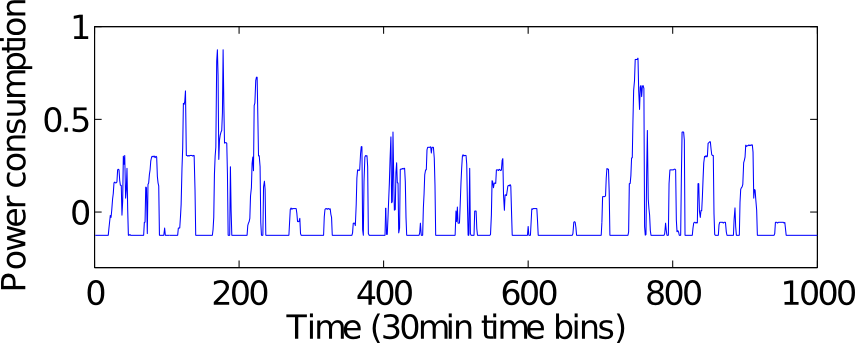
\includegraphics[width=.4\textwidth]{figs/26.png}}
%  \subfigure[GHP trace]{\label{fig:raw_ghp}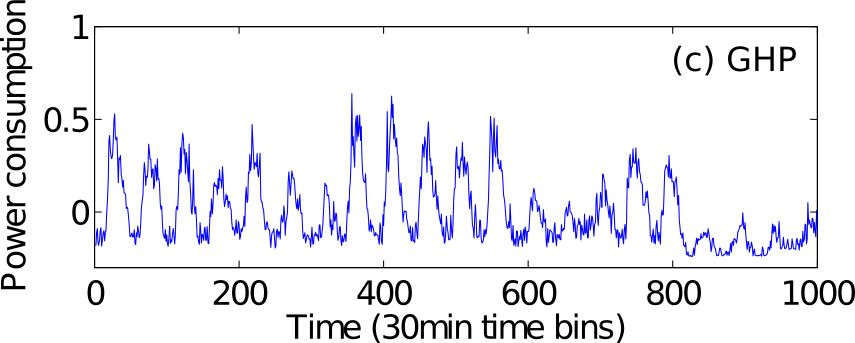
\includegraphics[width=.4\textwidth]{figs/41.png}}
%  \caption{Traces from three different sensors captured in 2011 from July 4th to July 24th. Data is normalized and aggregated into 30 minutes time bins.}
%  \label{fig:raw}
% \end{figure}


\subsection{Sutardja Dai Hall Analysis Methodology}
The methodology used in the SDH is more extensive and consists of several steps. Each is discussed in great details
in this section.

\subsubsection{Distribution Analysis}
For the second part of our evaluation, we perform an empirical study on sensor data collected from 15 sensors across 5 rooms. 
Each room has three sensors: a temperature sensor, a $CO_{2}$ sensor,  and a humidity sensor. 
The data from these is reported to an  
sMAP~\cite{smap} archiver. The data set used comes from two separate deployments: one is a deployment~\cite{Jay} lasting 
over 6 months on several floors in Sutardja Dai Hall (SDH) at UC Berkeley, where one sensor box -- which contains a thermometer, a humidity sensor
 and a $CO_{2}$ sensor -- is placed in each room. The box reports data over 6LowPAN~\cite{6lowpan} to a sMAP archiver every 
 15 seconds. The other is a long-term deployment comprised of thousands of sensors in dozens of buildings on campus. 
 We choose the portion of the SDH data set where the sensor devices, accessible via BACnet, report data to the archiver every few minutes. 
 Due to intermittent data loss, we pick a time span without interruption, starting in January until mid-February, 2013, for evaluation.

Let $ts^{i}_{j,t}$ be a time-series for sensor $j$ in room $i$ observed over some time interval $t$.  For simplicity, we ignore
$t$ in defining subsequent functions and re-introduce it where necessary.
For each trace we run EMD and obtain a set of $n$ IMFs, denoted as follows:
 % and applying EMD on such a trace will produce,
\begin{displaymath}
\Phi^i_j = EMD(ts^i_j) = \left \{ IMF_{1\sim n} \right \}
\end{displaymath}

IMFs are traces themselves, so we divide and re-aggregate them into the four bands $B$.
% further described in Section~\ref{sec:aggr}.
\begin{displaymath}
B = \left \{ H(igh), M(edium), L(ow), R(esidue) \right \}
\end{displaymath} 

Let the re-aggregation of the bands be denoted as:
\begin{displaymath}
Aggr(\Phi^i_j) = \left \{ IMF^i_{f,j} \right \}
\end{displaymath} 

where $f \in B$.  We pick the \emph{medium} frequency band ($M$) to compute the pairwise corrcoeff of the sensor traces. 
In order to understand and characterize the boundary between sensors we consider two sets of corrcoeffs for each room; the ``intra"-room set and 
``inter"-room set, as defined:
\begin{displaymath}
R^{i}_{intra,t} = \left \{ r(IMF^{i}_{M,j,t}, IMF^{i}_{M,k,t}) \right \}, \,
s.t.\, \forall j,k \in S_i
\end{displaymath}

The intra set only contains pairs of sensors in the same room, so both $ts^{i}_{j,t}$ and $ts^{i}_{k,t}$ are traces from 
sensors in room $i$.
\begin{displaymath}
R^{i}_{inter,t} = \left \{ r(IMF^{i}_{M,j,t}, IMF^{i'}_{M,k,t}) \right \},
\end{displaymath}
\begin{displaymath}
s.t. \, \forall j \in S_i, \, \forall k \in S_i', \, i \neq i' 
\end{displaymath}

By contrast, the \emph{inter} set contains pairs across rooms, meaning $ts_{j,t}$ is a trace from a sensor in room $i$ and 
$ts_{k,t}$ is a sensor trace from some other room $i'$.  %, and $t$ is the time span of the sensor trace the IMFs are derived from.
Note the use of $t$ in the definitions.  We re-introduce $t$ here to denote that the construction of each set is performed with respect to a specific time interval.

Finally, we examine populations, $R^i_{intra}$ and $R^i_{inter}$, across multiple time intervals (in days):%which are defined as,
\begin{displaymath}
R^{i}_{intra} = \bigcup_{\forall t}^{} R^i_{intra, t}, \; s.t. \; t \in \left \{ 1,3,5,7,14,21,28\right \}
\end{displaymath}

\begin{displaymath}
R^{i}_{inter} = \bigcup_{\forall t}^{} R^i_{inter, t}, \; s.t. \; t \in \left \{  1,3,5,7,14,21,28\right \}
\end{displaymath}

We generate a CDF for each of the two populations with respect to each room.  
This allows us to closely examine the statistical characteristics 
of the relationship between sensors in the same space and those in different spaces.  Each room offers a potentially different 
perspective on this relationship.


\subsubsection{Threshold Analysis}
In order to understand the statistical properties, we generate two corrcoeff distributions by computing the corrcoeff between pairs of traces within and across each room, as detailed in the previous section.
Figure~\ref{fig:group} shows how we divide the corrcoeff values into two sets.
The figure shows two intra and two inter sets. Specifically, we examine how a choice in cut-off threshold affects the ability
to separate the sets, when their separation is not known a priori, relative to each room.
Our hypothesis is that there exists a computable, statistical boundary between sensors in different rooms.

To test our hypothesis, we choose a threshold value relative to the distribution of corrcoeffs.  
All pairs with a corrcoeff larger than the threshold will be classified as being in the same room.  To closely analyze the threshold parameter, 
we generate a receiver operating characteristic (ROC) curve by varying the threshold value.  Then, we look for a good tradeoff point between the true-positive and false-positive rate; one that maximizes the difference between TPR and FPR.  We compare the ROCs generated 
for our ``medium'' frequency band IMFs against raw-signal, cross-correlation values, in order to ascertain the extent to which 
the SBS~\cite{SBS} methodology is advantageous for discovering a statistical separation, analogous to a physical one.
We also examine whether there is a uniform boundary between clusters across all the rooms. 


\begin{figure}[ht!]
\centering
	 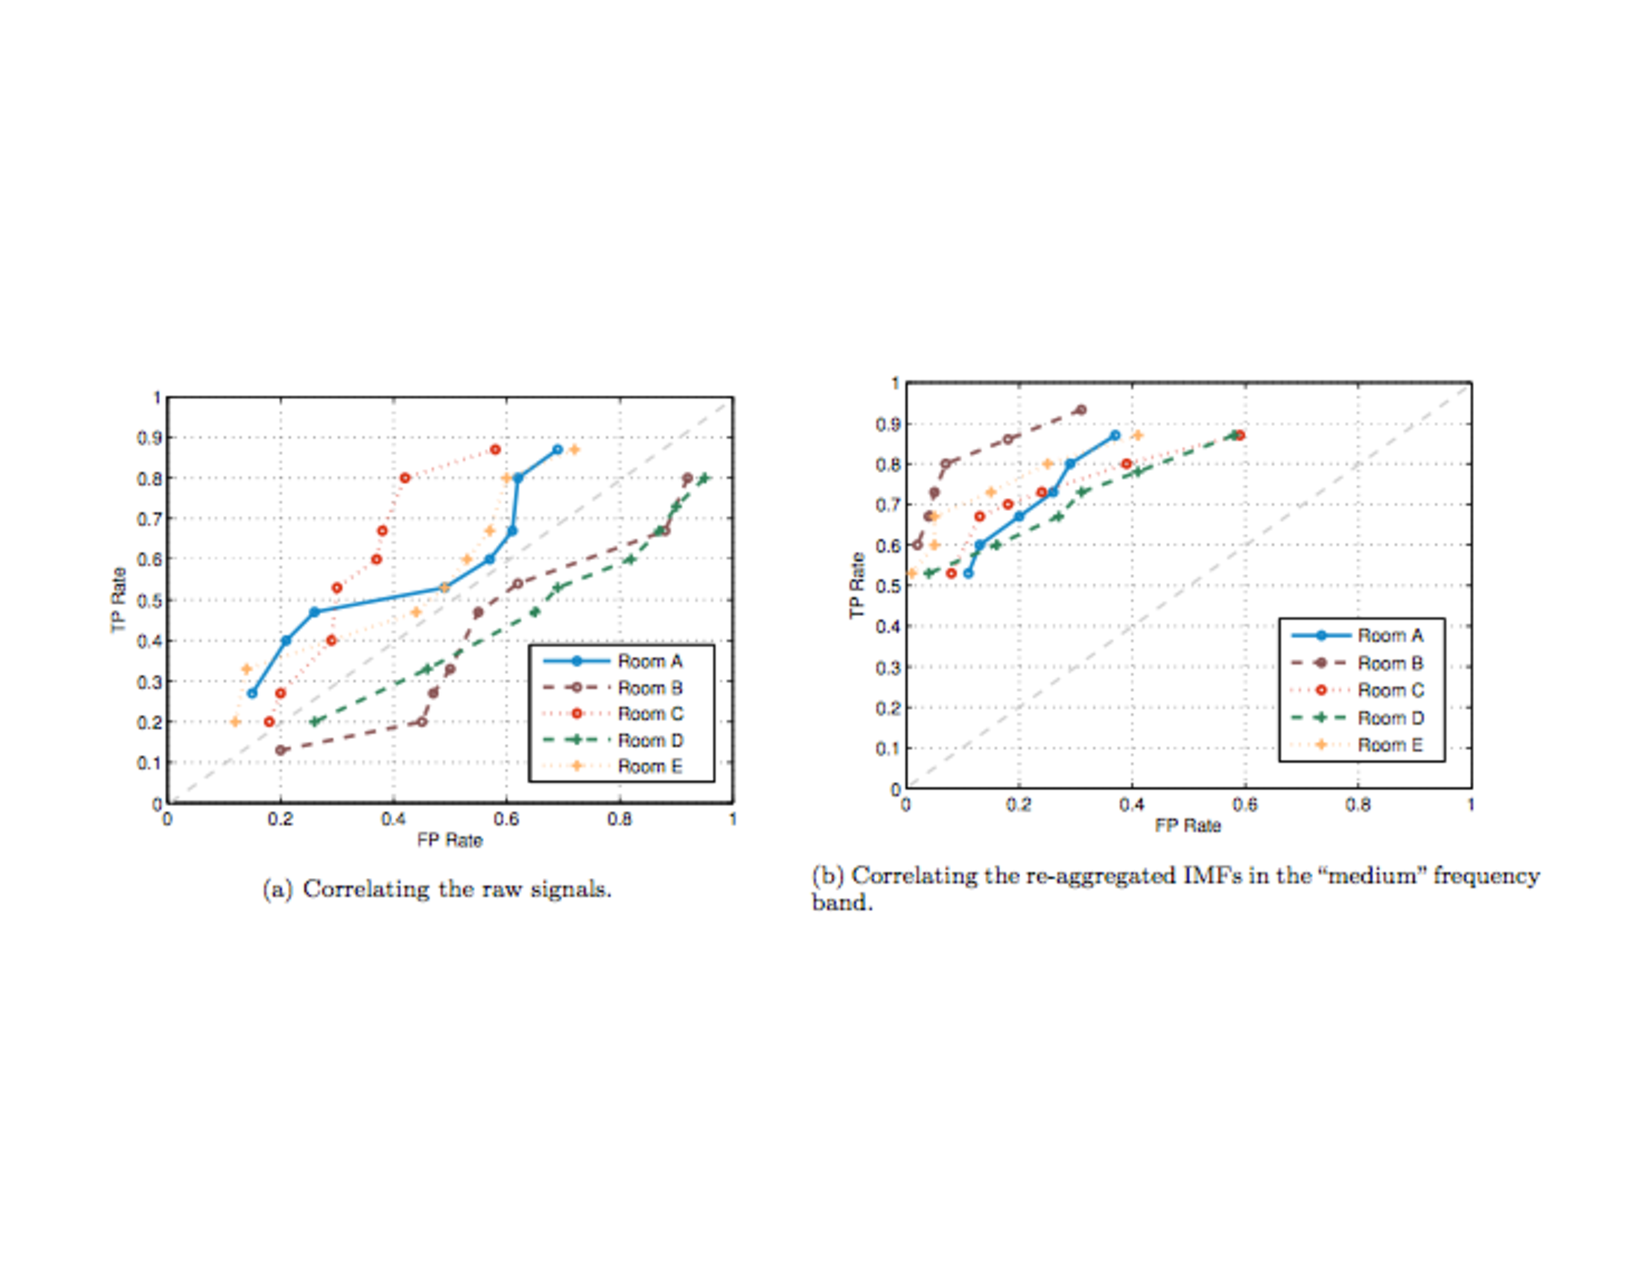
\includegraphics[width=1.00\textwidth]{figs/ROCgraphs}
\caption{The ROC curves depict the sensitivity of the raw signal and mid-frequency IMFs to the threshold value. We choose the 0.2 FPR point as the boundary threshold for each room. }
\label{fig:roc}
\end{figure}



\subsection{Experimental Setup}
\begin{figure}[h!]
\centering
  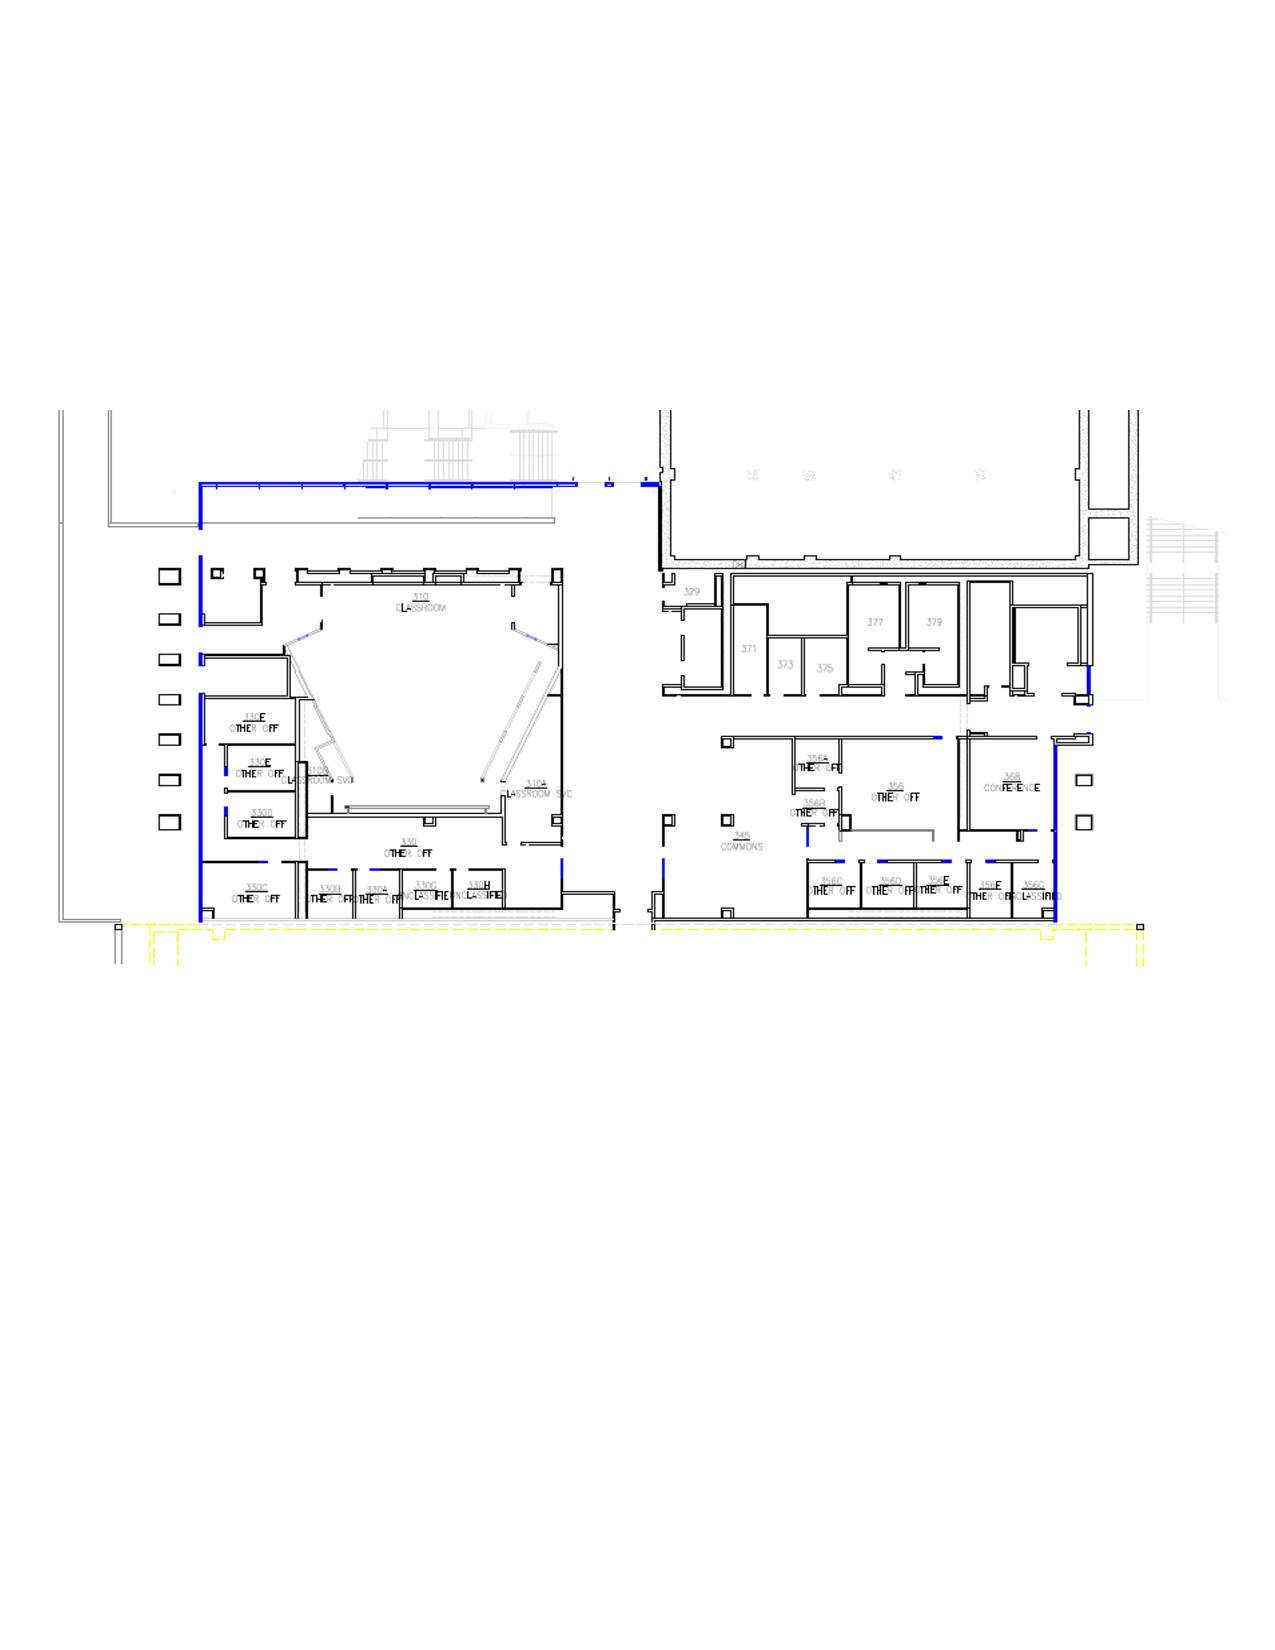
\includegraphics[width=0.45\textwidth]{figs/SDH3_crop}
\caption{We collect data from 15 sensors in 5 rooms sitting on 4 different floors. This is a map of a section of the 3rd floor
in Sutardja Dai Hall.}
\label{fig:sdh}
\end{figure}

We perform an empirical study on sensor data collected from 15 sensors across 5 rooms on 4 different floors of a Sutardja Dai Hall, 
as detailed in Table~\ref{table:roomspec}. 
Each room has three sensors: a temperature sensor, a $CO_{2}$ sensor,  and a humidity sensor. 
The data from these is reported to an sMAP~\cite{smap} archiver. The data set used comes from a deployment~\cite{Jay} lasting 
over 6 months on several floors in Sutardja Dai Hall (SDH) at UC Berkeley, where one sensor box -- which contains a thermometer, 
a humidity sensor and a $CO_{2}$ sensor -- is placed in each room. The box reports data over 6LowPAN~\cite{6lowpan} to a sMAP archiver 
every 15 seconds. 
Due to intermittent data loss, we pick a time span without interruption, starting in January until mid-Feburary, 2013, for evaluation.

\begin{table}[ht!]
\caption{Room Specs}
\centering % used for centering table
\begin{tabular}{c c c c}% centered columns (4 columns)
\hline %inserts single horizontal lines
Room\# & Orientation & Floor & Type \\ % inserts table 
%heading
\hline\hline % inserts double horizontal line
A & West & 2 & Computer Lab \\ % inserting body of the table
B & South & 4 & Conference Room \\
C & No Window & 2 & Classroom \\
D & North & 7 & Conference Room \\
E & South & 5 & Conference Room \\ % [1ex] adds vertical space
\hline %inserts single line
\end{tabular}
\label{table:roomspec} % is used to refer this table in the text
\end{table}

